\section{Optix: движок трассировки лучами общего назначения}
\begin{figure}[h]
\center{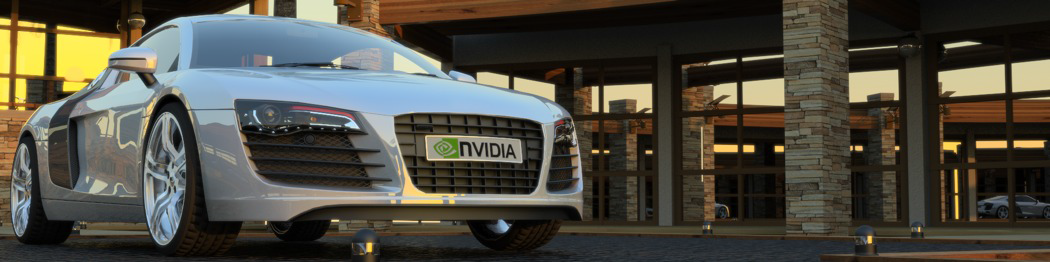
\includegraphics[width=1\linewidth]{audi.png}}
\caption{Изображение из приложения созданого в OptiX.}
\label{audi}
\end{figure}
\subsection{Краткий обзор}
Механизм трассировки лучей NVIDIA® OptiX™ --- программируемая система, разработанная для графических ускорителей NVIDIA и других массивно-параллельных архитектур.
Механизм OptiX основывается на базовом наблюдении, что большинство алгоритмов трассировки лучей могут быть реализованы, используя маленький набор программируемых операций. 
Следовательно, ядро OptiX --- проблемно-ориентированный JIT компилятор, который генерирует пользовательские ядра трассировки лучей, комбинируя предоставленные пользователями программы для генерации луча, заливки материала, объектного пересечения и обхода сцены. 
Оно включает реализацию очень широкого набора основанных на трассировке лучей алгоритмов и приложений, включая интерактивный рендеринг, оффлайн рендеринг, системы обнаружения коллизий, запросы искусственного интеллекта и научного моделирования, такие как звуковое распространение. 
OptiX достигает высокой производительности через компактную объектную модель и применения нескольких специфичной для трассировки лучей оптимизаций компилятора. 
Для простоты использования OptiX представляет модель программирования единственного луча с полной поддержкой рекурсии и динамического механизма отправки, подобного вызовам виртуальной функции.

\subsection{Введение}
Чтобы решить проблему создания доступной, гибкой, и эффективной системы трассировки лучей для массивно-параллельной архитектуры, представляем OptiX --- механизм трассировки лучей общего назначения. 
Этот механизм комбинирует программируемый конвейер трассировки лучей с легким представлением сцены. 
Общий интерфейс программирования включает реализацию множества основанных на трассировке лучей алгоритмов в графических и неграфических доменах, таких как рендеринг, звуковое распространение, обнаружение коллизий и искусственный интеллект.

В этом разделе мы обсуждаем цели проекта OptiX, а также реализации для NVIDIA Quadro®, GeForce® и Tesla® GPUs. 
Мы рассмотрим проблемно-ориентированную компиляцию с гибким набором средств управления иерархией сцены, ускоряющего создания структуры и обхода, непрерывного обновления сцены и динамично сбалансированной с загрузки модели выполнения GPU. 

Чтобы создать систему для широкого диапазона задач трассировки лучей, были принято несколько компромиссов и проектных решений, которые привели к следующим особенностям:
\begin{itemize}
 \item Общий низкоуровневый механизм трассировки лучей. 
 Механизм OptiX фокусируется исключительно на фундаментальных вычислениях, требуемых для трассировки лучей, и избегает встраивания конструкции для рендеринга. 
 Движок представляет механизмы для выражения взаимодействий геометрии луча и не имеет встроенного понятия световых сигналов, теней, коэффициента отражения, и т.д.

\item Программируемый конвейер трассировки лучей. 
Механизм OptiX демонстрирует, что большинство алгоритмов трассировки лучей может быть реализовано, используя маленький набор легких программируемых операций. 
Это определяет абстрактную модель выполнения трассировки лучей, поскольку последовательность пользователя определила программы. 
Эта модель при объединении с произвольными данными, хранившимися с каждым лучом, может использоваться, чтобы реализовать множество сложных графических сцен и невизуальных алгоритмов.

\item Простая модель программирования. 
Механизм OptiX обеспечивает такие механизмы выполнения, что программисты пользуются знакомыми методами работы с трассировкой лучами и  не обременяют себя низкоуровневой оптимизацией. 
Движок представляет знакомую рекурсивную, модель программирования единственного луча, а не пакеты луча или явные конструкции SIMD-стиля. 

\item Проблемно-ориентированный компилятор. 
Механизм OptiX комбинирует своевременные методы компиляции со специфичным для трассировки лучей знанием, чтобы реализовать его модель программирования эффективно. 
Абстракция механизма разрешает компилятору настраивать модель выполнения для доступных системных аппаратных средств.

\item Эффективное представление сцены. 
Механизм OptiX реализует объектную модель, которая использует динамическое наследование, чтобы упростить компактное представление параметров сцены. 
Гибкая система графика узла позволяет сцене быть организованной для максимальной производительности, все еще поддерживая инстанцирование, многоуровневую детализацию и вложенные ускоряющие структуры.

\end{itemize}


\subsection{Программируемый конвейер трассировки лучей}
Центральная идея механизма OptiX состоит в том, что большинство алгоритмов трассировки лучей может быть реализовано, используя маленький набор программируемых операций. 
Это прямой аналог к программируемым конвейерам растеризации, используемым OpenGL и Direct3D. 
На высоком уровне те системы представляют абстрактный растеризатор, содержащий легкие обратные вызовы для штриховки вершины, обработки геометрии, составления мозаики и операций штриховки фрагмента. 
Ансамбль этих типов программ, обычно используемых в многократных передачах, может использоваться, чтобы реализовать широкий спектр основанных на растеризации алгоритмов. 
 
Мы идентифицировали соответствующее абстрактное выполнение трассировки лучей модель вместе с легкими операциями, которые могут быть настроены реализовывать большое разнообразие основанных на трассировке лучей алгоритмов.[NVIDIA 2010a]. 
Эти операции или программы, могут быть объединенны с определяемой пользователем структурой данных (payload), связанной с каждым лучом. 
Ансамбль программ действует сообща для реализации алгоритма определенного клиентского приложения.

\subsubsection{Программы}
Есть семь различных типов программ в OptiX, каждая из которых работает над одним лучом одновременно.
Кроме того, программа ограничительной рамки действует на геометрию, чтобы определить границы примитива для построения ускоряющей структуры.
Сочетание пользовательских программ и жестко закодированного OptiX ядра образует конвейер трассировки лучей, который описан на рисунке~\ref{fig:graph-of-calling}. 
В отличие от конвейера прямой подачи растеризации более естественно думать о конвейере трассировки лучей как о графе вызовов.
Основная операция, rtTrace, чередуется между поиском пересечения (Traverse) и реагированием на этой пересечение (Shade).
При записи или чтении данных в объявленном пользователем payload луча и в массивах глобальной памяти устройства (буферы), эти операции объединяются для выполнения произвольных вычислений во время трассировки лучей.

Программы генерации лучей являются начальной точкой в конвейере трассировки лучей.
Один вызов rtContextLaunch создаст много экземпляров этих программ.
В примере на рисунке 3 программа генерации луча создает луч с использованием модели камеры pinhole для одного пикселя, начинает операцию трассировки и сохраняет результирующий цвет в выходной буфер.
 С помощью этого механизма, можно также выполнять другие операции, такие как создание фотонных карт, вычисления освещения методом отжига, обработки запросов лучей, переданных из OpenGL, стрельба несколькими лучами для суперсемплинга или реализации различных моделей камер.
Программы пересечения реализуют тесты пересечения лучевой геометрии.
При пересечении ускоряющих структур система будет вызывать программу пересечения, чтобы выполнить геометрический запрос.
Программа определяет, и где луч касается объекта и может вычислять нормали, текстурных координат, или другие атрибуты в зависимости от положения попадания.
Произвольное количество атрибутов могут быть связаны с каждым пересечением.
Программы пересечения включают поддержку произвольных поверхностей, таких как сферы, цилиндры, поверхностей высокого порядка, или даже фрактальной геометрии, как множество Жюлиа.
Тем не менее, даже в системах,состоящих только из треугольников, можно встретить большое разнообразие представлений сетки.
Программируемая операция пересечения облегчает прямой доступ в оригинальном формате, который может помочь избежать копии при взаимодействии с системами на основе растеризации.
\begin{figure}[h]
\center{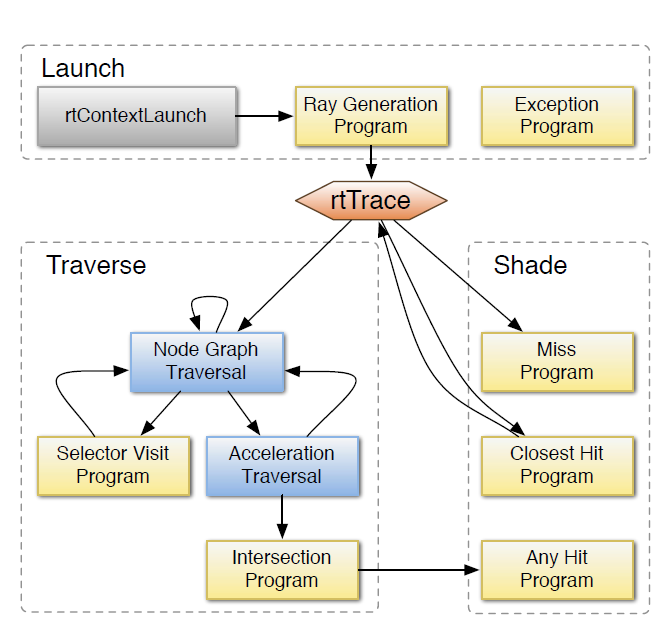
\includegraphics[width=0.7\linewidth]{fig.png}}
\caption{Граф вызова, показывающий поток управления по конвейеру трассировки лучей.Желтые прямоугольники представляют указанные пользователем программы, а синие прямоугольники ---алгоритмы внутренние для OptiX.
Выполнение инициируется вызовом API rtContextLaunch.Встроенная функция, rtTrace, может быть использована в программе генерации лучей для отправки лучей в сцену.
Эта функция также может вызываться рекурсивно программой ближайшего попадания для тени и вторичных лучей.
Программа исключения выполняется, когда выполнение отдельного луча завершилось с ошибкой, такой как чрезмерное потребление памяти.}
\label{fig:graph-of-calling}
\end{figure}

Программы ограничительной рамки вычисляют границы, связанные с каждым примитивом для включения ускоряющей структуры над произвольной геометрией.
Учитывая примитивный индекс, простая программа такого типа может, например, читать вершинные данные из буфера и вычислять треугольники ограничительной рамки.
Процедурная геометрия может иногда только оценить границы примитива.
Такие оценки допускаются пока они консервативны, но свободные границы могут привести к снижению производительности.

Ближайшие программы попадания вызываются один раз обхода нашла ближайший  пересечение луча с геометрии сцены.
 Этот тип программы очень напоминает поверхностный шейдеров в классических системах визуализации.
 Как правило, программа ближайшего попадания будет выполнять вычисления, такие как затенение, потенциальное излучение новых лучей в процессе, и сохранение результирующих данных в payload луча.

Программы любого попадания вызываются во время обхода для каждого пересечения объекта луча, который находится.
Программа любого попадания позволяет материалу участвовать в решении объектного пересечения, сохраняя при этом операции затенения отдельно от операций геометрии.
Она необязательно может завершить луч с помощью встроенной функции rtTerminateRay, которая будет останавливать все обходы и освободить стек вызовов до самого последнего вызова rtTrace.
Это легковесный механизм исключение, который может быть использован для реализации раннего обрыва теневых лучей и пространственной непроходимости.
Кроме того, программа любого попадания может игнорировать пересечение используя rtIgnoreIntersection, которая позволяет обходу продолжать искать другие геометрические объекты.
Пересечение может быть проигнорировано, например, на основе текстуры поиска канала, тем самым реализация эффективной альфа-прозрачности отображается без перезагрузки обхода.
\begin{figure}[h]
\begin{verbatim}
RT_PROGRAM void pinhole_camera() {
Ray ray = PinholeCamera::makeRay( launchIndex );
UserPayload payload;
rtTrace( topObject, ray, payload );
outputBuffer[launchIndex] = payload.result;
}
\end{verbatim}
\caption{Пример программы генерации луча (в CUDA C) для одного сэмпла на пиксель.
Расположение 2-мерной сетки вызова программы дает семантическую переменную launchIndex, которая используется для создания первичного луча с помощью модели pinhole камеры.
Во время трассировки луча, вызванные программы попадания материала заполняют результирующее поле в определяемой пользователем структуре payload.
Переменная topObject указывает на месторасположение в иерархии сцены, где луч обхода должен начинаться, как правило, в корне узла графа.
На месте, указанном launchIndex, результат записывается в выходной буфер, который будет отображаться в приложении.}
\end{figure}

  Программы промаха выполняются, когда луч не пересекает любую геометрию в предоставленном интервале.
  Они могут быть использованы для реализации цвета фона или подстановки карты среды .

  Исключение программы выполняются, когда система обнаруживает состояние исключения, например, когда стек рекурсии превышает объем памяти, доступный для каждого потока, или когда индекс доступа к буферу вне диапазона.
  OptiX также поддерживает определяемые пользователем исключения, которые могут быть сгенерированы из любой программы.
  Программа исключение может реагировать, например, с помощью печати диагностических сообщений или визуализации состояний путем записи специальных цветовых значений в буфер вывода пикселя.
  Программы выбора обхода подвергаются программированию для низкого уровня узла обхода графа.
  Например, приложение может выбрать изменение уровня геометрической детализации для частей сцены на Perray основе.
  В этом случае, программа выбора будет рассматривать расстояние лучей или дифференциал лучей, который хранится с полезной нагрузкой и принимает решение обхода на основе этих данных.
  
 \subsubsection{Представление сцены}
 
 Движок OptiX использует гибкую структуру для представления информации сцены и связанные программируемые операций, собранные в объекте контейнера называнные контекстом.
 Это представление тоже является механизмом для привязки программируемых шейдеров к данным конкретного объекта, которые требуются.

\paragraph{Узлы иерархии.}

Сцена представлена как график. Это представление очень легковесное и управляет обходом лучей через сцену. 
 Оно также может быть использовано для реализации двухуровневой иерархии сущностей для анимации твердых предметов или других общих структур сцены.
 Для поддержки создания экземпляров и обмена общими данными, узлы могут иметь несколько родителей.
 Четыре основных типов узлов могут быть использованы, чтобы обеспечить представление сцены с помощью ориентированного графа.
 Любой узел может быть использован в качестве корневого узла обхода.
 Это позволяет, например, создавать различные представления, которые будут использоваться для различных типов лучей.
 
Группа узлов содержать ноль или более (но обычно два или больше) потомков любого типа узла.
Узел группы имеет структуру ускорения, связанный с ним, и может быть использовано, чтобы обеспечить верхний уровень структуры двухуровневого обхода.
Геометрическая группа узлов является потомками на графике и содержат примитивные и материальные объекты, описанные ниже.
Этот тип узла также имеет структуру ускорения связанную с ним.
Любая непустая сцена будет содержать хотя бы одну геометрическую группу.
Преобразованные узлы имеют один дочерний элемент любого типа узла, а также связанную матрицу $4 \times 3$, которая используется для выполнения преобразованиz базовой геометрии.
Выбранные узлы имеют ноль или более потомков любого типа узла, плюс одну программу обхода, которая выполняется для выбора среди имеющихся потомков.
Хотя это и не реализовано в текущей версии Optix библиотек, узел граф может быть циклическим, если узел селектора использовать осторожно, чтобы избежать бесконечной рекурсии.

\paragraph{ Геометрические и материальные объекты.}

Основная часть данных хранится в геометрии узлов в потомках графа.
Они содержат объекты, которые определяют геометрию и затенение операции.
Они могут также иметь несколько родителей, позволяя материалам и геометрии осуществлять обмен информацией в нескольких точках на графе.

Объекты Геометрической сущности связан с геометрическим объектом набором материальных объектов.
Это общая структура, используемая графами сцены позволяет сохранить геометрическую и теневую информацию ортогонально.

Объекты материала храненят информацию о операциях затенения, включая программы, вызываемые для каждого пересечения по мере их обнаружения (программа любого попадания) и для ближайшего пересечения к началу данного луча (программа ближайшего попадания).

\begin{figure}[h!]
\center{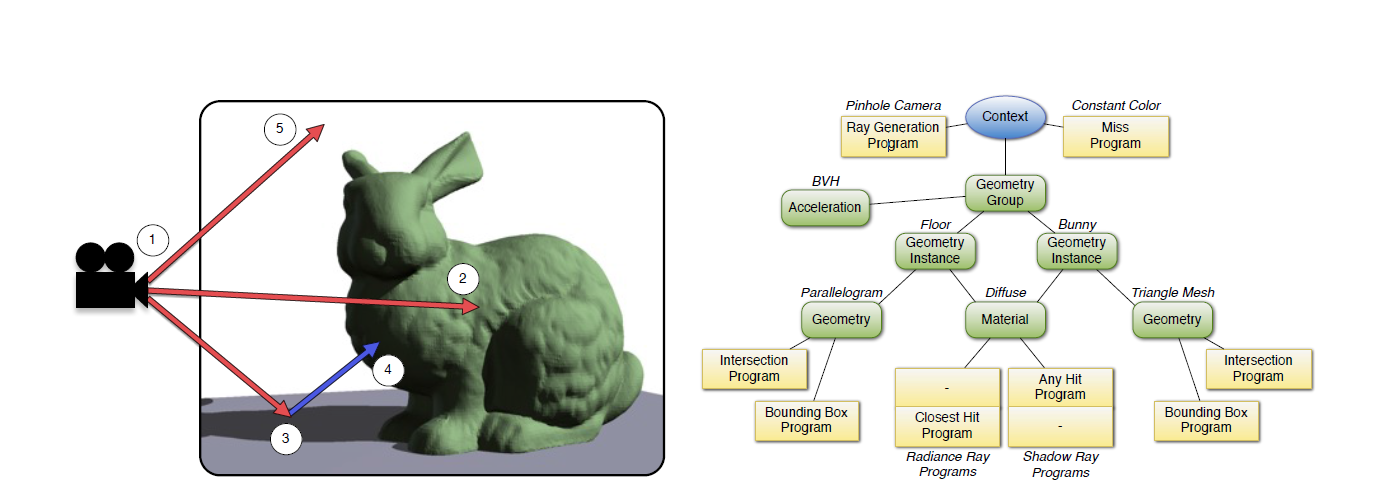
\includegraphics[width=1\linewidth]{fig1.png}}
\caption{Справа: Полный контекст OptiX простой сцены с помощью pinhole камеры, двух объектов и теней.
Программа генерации луча реализует камеру, в то время как программа промаха реализует постоянный белый фон.
Геометрия одной группы содержит два сущности геометрии с одной BVH построеной через всю основную геометрию в треугольной сетке и плоскостях.
Два типа геометрии будут реализованы, треугольная сетка и параллелограмм, каждый со своим набором пересечения и программе ограничивающей рамки.
Два экземпляра геометрии совместно используют один материал, который реализует диффузную модель освещения и полностью ослабляет теневые лучи через программы ближайшего попадания и любого попадания соответственно.
Слева: Выполнение программ. 1. Программа генерации луча создает лучи и проводит их через группы геометрии, который инициирует BVH обход.
2. Если луч пересекается с геометрией,программа ближайшего попадания будет вызываться после того как точка попадания будет найдена.
3. Материал будет порождать теневые лучи и простраивать их от геометрии сцены.
4. Когда пересечение вдоль теневого луча найдено, программа любого попадания прекращает обход луча и возвращает в вызывающую программу с информацией о тени.
5. Если луч не пересекает с какой-либо геометрией сцены, будет вызываться программа промаха.}
\label{fig1}
\end{figure}

\subsubsection {Объектная модель и модель данных}
OptiX использует объектную модель специального назначения, предназначенную для минимизации постоянных данных, используемых в программных операциях.
В отличие от системы OpenGL, где только одна комбинация шейдеров используется одновременно.
Тем не менее, трассировка лучей может случайно получить доступ к данным материала и объекта. Поэтому вместо общих переменных, используемых в шейдерных языках OpenGL, OptiX позволяет описать любой объект и узел, описанный выше задав произвольный набор переменных, выраженных как пара ключ-значение.
Переменные устанавливаются клиентским приложением и имеют доступ только для чтения во время выполнения трассировки.
Переменные могут быть скалярного или векторного целого типа или с плавающей точкой (например, float3, int4), а также определяемые пользователем Структуры и ссылки на буферы и текстурные образцы.

Механизм наследования для этих переменных является уникальным для OptiX.
Вместо основных классов модели наследования с одной сущностью или указателем на него, движок OptiX отслеживает текущую геометрию и материальные объекты и текущий узел обхода.
Значения переменных наследуются от объектов, которые являются активными в каждой точке потока управления.
Например, программа пересечения унаследует определения от геометрии и геометрических объектов, в дополнение к глобальным переменным, определенным в контексте.
Концептуально, OptiX рассматривает каждый из этих объектов как пару ключ / значение, когда есть доступ к переменным.
Этот механизм, который можно рассматривать как обобщение вложенной области видимости, можно найти в большинстве языков программирования. Он также может быть реализован достаточно эффективно в JIT компиляторе.

В качестве примера, как это используется, рассмотрим массив источников света, называемых светом.
Как правило, пользователь будет определять свет в контексте, общий OptiX.
Это присваивает данное значение для всех шейдеров в всех сценах.
Однако, если свет для конкретного объекта необходимо переопределить, другая переменная с этим же именем может быть создана и присоединена к экземпляру геометрии, связанной с этим объектом.
Таким образом, программы, связанные с этим объектом будет использовать переопределенное значение света, а не значения, прикрепленное к контексту.
Это мощный механизм, который может быть использован для минимизации данных сцены, что обеспечивают высокую производительность на архитектурах с минимальными кэшем.
Манера, в которой обрабатываются эти случаи может значительно варьироваться от одной визуализации к другой, так что движок OptiX обеспечивает базовую функциональность, чтобы выразить любое количество правил переопределения эффективно.

Особый тип переменной, отмеченного атрибутом ключевых слов можно использовать для передачи информации из программы пересечения с программой ближайшего и любого попадания.
Они аналогичны varying variables в OpenGL, и используются для передачи текстурных координат, нормалей и другой информации о затенении от программ пересечения к программами затенения.
Эти переменные имеют специальную семантику-они написаны программой пересечения, но только хранятся значения, связанные с ближайшей точкой пересечения.
Этот механизм позволяет операциям пересечения быть полностью отделеными от операций затенения, включая несколько подобных примитивов и / или сетки форматов хранения в то же время поддерживая текстурирование, затенение нормалейи и объектов кривизны для разносных лучей.
Атрибуты, которые не используются любой программой ближайшего или любого-попадания могут быть опущены компилятором OptiX.

\subsubsection {Динамическая отправка}
Чтобы позволить нескольким операциям трассировки лучей сосуществовать в одном исполнении, OptiX использует пользовательский тип луча.
Тип луча это просто индекс, который выбирает определенный набор слотов для программ любого и ближайшего попадания, который будет выполнен, если точка пересечения найдена.
Это может быть использовано, например, для обработки теневых лучей отдельно от других лучей.

Точно так же, несколько точек входа в контексте OptiX включают эффективный способ представлять различные проходы по тем же набором геометрии.
Например, маппер фотона может использовать одну точку входа, чтобы излучить фотоны в сцену и вторую точку входа для просмотра излученных лучей.

\subsubsection{Буферы и текстуры}
Ключевая абстракция для хранения больших объемов данных является объектом многомерного буфера, который представляет собой 1 -, 2 - или 3-мерный массив фиксированного размера элемента.
Буфер можно получить через объект C+ + обертки в любой из программ.
Буферы могут быть доступны только для чтения, только для записи или для чтения и записи и поддерживать атомарные операции, когда поддерживаются аппаратно.
Буфер основанный на дескрипторе не предоставляет необработанные указатели, что позволяет среде выполнения OptiX в реальном времени переразмещать буферы для хранения уплотнения, или для продвижения к другим пространствам памяти для производительности.
Буферы обычно используются для вывода изображений, данных треугольников, списков источников света и других данных на основе массивов.
Буферы являются единственным средством вывода данных из программы OptiX.
В большинстве случаев, программа генерации луча будет отвечать за запись данных в выходной буфер, но любой из программ Optix разрешается писать в выходные буферы в любом месте, но без каких-либо гарантий очередности.
Буфер также может быть привязан к объекту текстурного сэмплера, который будет использовать аппаратное GPU текстурирование.
Буферы и объекты текстурного сэмплера обязаны быть Optix переменными и использовать те же механизмы сбора данных как шейдерных значений.
Кроме того, оба буфера и блока выборки могут взаимодействовать с OpenGL и DirectX, включая эффективную реализацию гибридных растеризации / трассировки лучей приложения.

